\chapter{Cart-Pole \& Mountain-Car}
\section{Cart-Pole}
The cart-pole environment, which is an implementation of the famous cart-pole problem [7], is a popular AI benchmark that simulates a pole that needs to be balanced on the flat rectangle (cart) that it's attached to. The observation object of this environment includes the velocity and position of the cart, the velocity at the tip of the pole, and the angle of the pole. Initially, these parameters are assigned a random value in the range $[-0.05, 0.05]$, which results in the pole standing almost upright with a slight tilt. The environment only allows two discrete actions (left and right) which the agent uses to balance the pole before it falls over, by pushing the cart without causing it to go off-screen. The environment terminates if the agent fails in either of those tasks, or after the maximum number of time-steps (200) is reached. The agent receives $1$ reward on every time-step until one of these termination criteria is met. Finally, this environment is considered to be solved if the agent achieves an average reward of greater than or equal to $195.0$ over 100 consecutive trials. More details about the various environmental parameters can be found in the environment’s official GitHub Wiki page\footnote{\url{https://github.com/openai/gym/wiki/CartPole-v0}}.

\subsection{Experiment 1: Binary Programs}
The goal of the first experiment was to implement the simplest GP algorithm that performs better than a random agent. The simplest language that can encode the actions allowed in this environment is one of 0’s and 1’s, where 0’s represent ‘left’ and 1’s represent ‘right’. The program structure, therefore, included the terminal set \verb+T = {0, 1}+ and an empty function set. The intuition for this structure was that, in principle, there has to exist a string of left-right actions that manages to balance the pole on the cart most of the time. 

This GP agent did not managed to achieve better-than-random performance: a random agent achieves an average reward of $\approx22.0$ and the best programs the GP algorithm generated achieved an average reward of $16.76$. The most likely reason for this is that these programs are static, which means they don’t use information about the state of the environment to compute the next action to take. This limitation would not be a problem if the initial state of the environment was always the same, because that would make the state transitions deterministic and, therefore, there would exist a static program that would reliably balance the pole. However, the initial state of the environment is randomised each time the environment starts running and the range of possible values for the various parameters of the environment is sufficiently large, such that no static strategy can perform well.

\subsection{Experiment 2: Known Strategy}
The main goal of the second experiment was to enable the agent to utilise the environment state to choose actions dynamically. At the same time, I wanted to test the capabilities of the GP algorithm, since it would be used to find increasingly complex programs as the environments proved to be more difficult to solve. To achieve both of these goals, a manual strategy was discovered that performed well by utilising the environment state. The program structure of the GP algorithm was also adjusted to allow it to discover the strategy automatically. The chosen strategy can be described as follows:

\begin{verbatim}
    if pole_angle <= 0 then push_left() else push_right()
\end{verbatim}

Intuitively, this strategy describes the behaviour "if the pole is leaning to the left, push the cart to the left; if the pole is leaning to the right, push the cart to the right". This should keep the pole balanced at all times. To test this intuition, I implemented an agent that follows this strategy and tested it on the environment. The agent achieved an average score of $42.0$, a major improvement over the previous agent. Then, I introduced a simple environment-specific language to replace the binary language of the previous experiment, which included variables to represent the environment state and the actions the agent can take, flow-control (if-statements) and comparison operators to allow the agent to make decisions dynamically, and constants for calculations. The function and terminal set used for this experiment were \verb+F = {IFLTE}+ and \verb+T = {pa, 0, L, R}+ respectively.

The function set included a single function, \verb+IFLTE+ (if-less-than-or-equal), which accepts 4 inputs; if the first input is less than or equal to the second input, it outputs the third input; otherwise, it outputs the fourth input. This functionality seemed sufficient to encode the strategy described above. The terminal set included four elements: the pole angle (\verb+pa+) used to encode the corresponding environment observation, the numerical constant \verb+0+ which was required for the comparison performed in the strategy, and the actions \verb+L+ and \verb+R+, left and right respectively. The program structure was quite restricted in this first version of the algorithm to make it easier to evaluate and troubleshoot before applying it to more difficult environments that would require a more complex program structure. Specifically, each program was restricted to consist of a single \verb+IFLTE+ function, which could only accept \verb+pa+ and \verb+0+ as its first two arguments, and \verb+L+ and \verb+R+ as its third and fourth arguments (figure \ref{fig:iflte_tree}). It was important to restrict the third and fourth arguments to actions since the output of the program had to be the action the agent would perform in the environment. Therefore, a simple type system was implemented to perform this check. Using this simple functional language, the manually-discovered strategy could be encoded as \verb+IFLTE(pa, 0, L, R)+.

\begin{figure}[ht]
    \centering
    
\includegraphics[width=12cm]{images/simple_iflte_program.png}
    \caption{Tree representation of the program structure of the Known Strategy agent}
    \label{fig:iflte_tree}
\end{figure}

With these structural restrictions, it was easy for the GP algorithm to converge to the intended strategy (it only required a single generation, and mutation was not needed) because the program space was very small. The exact parameters used for the experiment are summarised in table \ref{tab:cartpole_exp2_params}.

\begin{table}[ht]
    \centering
    \begin{tabular}{|l|c|}
        \hline
        \textbf{Parameters} & \textbf{Values} \\
        \hline
        Population size     & 10  \\
        Max generations     & 5   \\
        Max program depth   & 1  \\
        Terminal fitness & 195.0 \\
        Number of runs      & 1   \\
        Number of episodes  & 100 \\
        Episode length      & 200  \\
        \hline
    \end{tabular}
    \caption{Experiment parameters (cart-pole experiment 2)}
    \label{tab:cartpole_exp2_params}
\end{table}

\subsection{Experiment 3: Exploration}
\subsubsection{Setup and Motivation}
The goal of the final experiment was to expand the program space to encourage exploration and allow the algorithm to discover better strategies than the one found manually. The terminal set was extended to include the second observation of the environment, pole velocity (\verb+pv+), to allow the algorithm to incorporate it in the solution. Additionally, I experimented with constants other than \verb+0+ and it turned out that the performance was very sensitive to even very small deviations from \verb+0+. Specifically, I discovered that including the constant \verb+0.025+ in the terminal set increased the performance of the discovered solutions significantly. Finally, the program structure was adapted to allow for the generation of programs that utilised higher-order functions (i.e. functions that accept functions as arguments) which can be represented as a trees of varying depth (see figure \ref{fig:deep_iflte_tree} for an example). The extended terminal set was \verb+T = {pa, pv, 0, 0.025, L, R}+. The parameters used for this experiment are summarised in table \ref{tab:cartpole_exp3_params}.

\begin{figure}[ht]
    \centering
    
\includegraphics[width=12cm]{images/complex_iflte_program.png}
    \caption{Tree representation of the program structure of the Exploration agent}
    \label{fig:deep_iflte_tree}
\end{figure}

\begin{table}[ht]
    \centering
    \begin{tabular}{|l|c|}
        \hline
        \textbf{Parameters} & \textbf{Values} \\
        \hline
        Population size     & 100  \\
        Max generations     & 5  \\
        Max program depth   & 2  \\
        Terminal fitness & 195.0 \\
        Number of runs      & 1   \\
        Number of episodes  & 100 \\
        Episode length      & 200  \\
        \hline
    \end{tabular}
    \caption{Experiment parameters (cart-pole experiment 3)}
    \label{tab:cartpole_exp3_params}
\end{table}

\subsubsection{Results and Discussion}
The initial results of this experiment showed that the second observation, pole velocity, was more useful than the pole angle, so programs using \verb+pv+ instead of \verb+pa+ tended to dominate the population during the first few generations. The first run of GP converged on the program \verb+IFLTE(pv, 0, L, R)+, which achieved an average reward of $181.78$. This improvement could be attributed to the fact that the velocity of the pole provided the agent with more useful information than its angle. Using the first strategy (\verb+IFLTE(pa, 0, L, R)+), if the pole leaned towards, say, the right at the beginning of the run, the agent would begin to push the cart to the right to cause the pole to lean towards the left, bringing it back to the center. The problem with this strategy was that by the time the pole angle became negative (meaning the pole leaned towards the left) it had accumulated too much momentum for the agent to manage to push left to balance it on time. The agent was essentially over-correcting. Using the new strategy, the agent detected which direction the pole was accelerating towards (using the sign of its velocity) and pushed the cart towards that direction for just long enough to prevent the pole from falling over, without over-correcting. However, this strategy was still problematic (as is evident from the imperfect score it achieved) because the agent stopped pushing the cart as soon as the sign of the pole velocity was flipped, so the pole didn't have enough momentum to lean towards the other side, thereby letting it fall towards the same side again. The result of this was that the agent was now under-correcting, balancing the pole perfectly, but at an angle, causing the cart to move until it eventually exited the screen and the environment terminated. It was evident at this point that a solution would involve information about both the pole angle and its velocity.

Increasing the maximum number of generations from 5 to 10 allowed for more complex solutions to arise. Eventually, the algorithm consistently produced solutions that achieved the reward specified as the solution criterion for the environment. These solutions included programs using nested if statements and combining both observation variables. An example of such a program is:
\begin{verbatim}IFLTE(0.025, pa, IFLTE(pv, pv, R, L), IFLTE(0.025, pv, R, L))\end{verbatim}
This program achieves an average reward of $198.74$ over 100 consecutive trials. The following is an equivalent, but more readable, version of the strategy described by this program:

\begin{verbatim}
if pa > 0.025 then R else (if pv > 0.025 then R else L)
\end{verbatim}

Following this strategy, the agent pushed the cart to the right to balance the pole if it was leaning at a right angle greater than some threshold ($0.025$). If the pole was leaning at a left angle or a small right angle, the agent checked the pole's velocity to make its decision: if the pole was accelerating towards the right (\verb+pv > 0.025+) then the agent pushed right to counteract it; otherwise it pushed left for the same reason.

This extended version of the program structure allowed the agent to achieve the goal of utilising exploration to find new and better solutions by exploring a larger program space. At this stage, the GP algorithm can incorporate new language extensions as well as additional genetic operators, both of which will be required in the following environments. So, Cart Pole was a useful starting point in showcasing the potential of this approach and establishing a framework for applying it to other RL environments.

\section{Mountain-Car}
The second RL environment attempted, was mountain-car. This environment simulates a car that attempts to climb a steep hill (figure \ref{fig:mountain-car}). There are two versions of this environment, one in which the actions the agent can take are discrete (similar to cart-pole) and one in which they are continuous (the action is a number that represents the magnitude of the force the agent applies to the car). The former is, in principle, easier to solve because there are fewer possible actions and, therefore, fewer strategies to explore before discovering a solution. The discrete version of the environment was attempted first with the hope that a solution to the simpler environment could be used as a basis for the more complex one.

\subsection{Experiment 1: Discrete Actions}
For the discrete version of this environment, I used the same parameters as in cart-pole experiment 3, and a similar program structure, adapted to the details of this environment:

\begin{verbatim}
F = {IFLTE}
T = {position, velocity, 0.0, 0, 1, 2}
\end{verbatim}
The terminals \verb+position+ and \verb+velocity+ represent the corresponding environment observations, \verb+0.0+ is a numerical constant used for comparisons (similar to cart-pole), and \verb+0+, \verb+1+, and \verb+2+ encode the discrete action space of the environment (push left, no action, and push right respectively).

In fewer than $10$ generations, the GP algorithm found the simple and intuitive program \\\verb+IFLTE(0.0, velocity, 2, 0)+, which achieves a fitness score of approximately $-120$, which is very close to the requirement for a solution, $-110$. This program encodes the strategy “if the velocity of the car is positive, push the car to the right (i.e. increase its velocity), otherwise push it to the left (i.e. decrease its velocity).” The agent effectively swings the car back and forth, maximising its momentum, until it can reach a high enough velocity to climb the hill and reach the goal. 

\subsection{Experiment 2: Continuous Actions}
The interpretable nature of the strategy found for the discrete version of this environment makes it reasonable to hypothesise that the same strategy should perform well on the continuous version of this environment. The same principle of applying a force proportional to the car’s velocity can be used, so the only required modification is changing the value of this applied force to a continuous value in the range $[0.0, 1.0]$, which defines the action space of this environment. 

The problem then becomes a simple numerical optimisation problem with one variable. Evaluating the program using all values in $[0.0, 1.0]$ with a $0.001$ increment, reveals that the optimal force is $0.180$, which produces an average fitness score of $98.80$, which is greater than the requirement for a solution ($90$). The complete set of results is visualised in figure \ref{fig:mountain_car_cont}, which shows that values between $0.0$ and $0.179$ produce negative fitness scores (the car is unable to reach the goal), and values after $0.180$ linearly decrease performance. The reason for the negative values at the beginning of the range is that the force applied to the car is not great enough to eventually allow it to climb the hill, so it only receives negative rewards from the environment on every time step. The optimal value is the smallest amount of force necessary to eventually allow the car to climb the hill, which satisfies the requirement of the environment (reaching the goal with the minimum amount of effort). Every value greater than the optimal increases the amount of effort beyond what is necessary for the goal to be achieved and, therefore, reduces the overall fitness score.

\begin{figure}[ht]
    \centering
    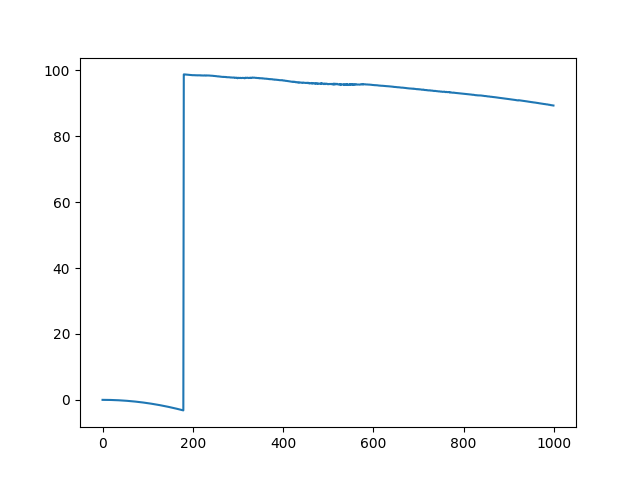
\includegraphics[width=12cm]{images/mountaincarcont.png}
    \caption{The x-axis represents the magnitude of the for applied to the car (multiplied by 1000) and the y-axis represents the average reward achieved using that magnitude.}
    \label{fig:mountain_car_cont}
\end{figure}

The simple and intuitive nature of this solution is further confirmation that GP is a suitable approach for solving (at least simple) RL environments. Another interesting feature of this program is its similarity to the solution for cart-pole, despite the differences between the environments. This is an indication that environments that share common characteristics (e.g. classic control environments) might be solvable using similar solutions.
